\label{chapter:related_work}

Given the similarities of GNNs with convolutional neural networks, one might be tempted to build deep graph neural networks. Breakthroughs in deep learning such as ResNet (\cite{he2015deep}) managed to build models with hundreds of layers, showing that improvement goes hand in hand with depth. Unfortunately, following the same course of action for GNNs does not seem to be beneficial for graph data, allthough they are often labeled as \textit{deep} learning methods. Most models, including the examples discussed in this report, only use a handful of layers and observe worse results with added depth.

Analysis of this issue has provided insight into a few phenomenas specific to the GNN domain. One of them is \textit{over-smoothing}. By adding more and more convolutional layers, a nodes' feature is influenced by a growing number of more distant neighbors. At some point, the receptive field of model is too large and causes all node features to converge to the same output, making it hard to distinguish between them \cite{oono2021graph}.

The effect of information loss with increased depth is even stronger when the neighborhood of a node grows rapidly within a few hops. In this case, there is too much information accumulated into the fixed-size feature vector of a node. This is the so-called \textit{bottleneck} phenomenon. 

\begin{figure}[h]
    \centering
    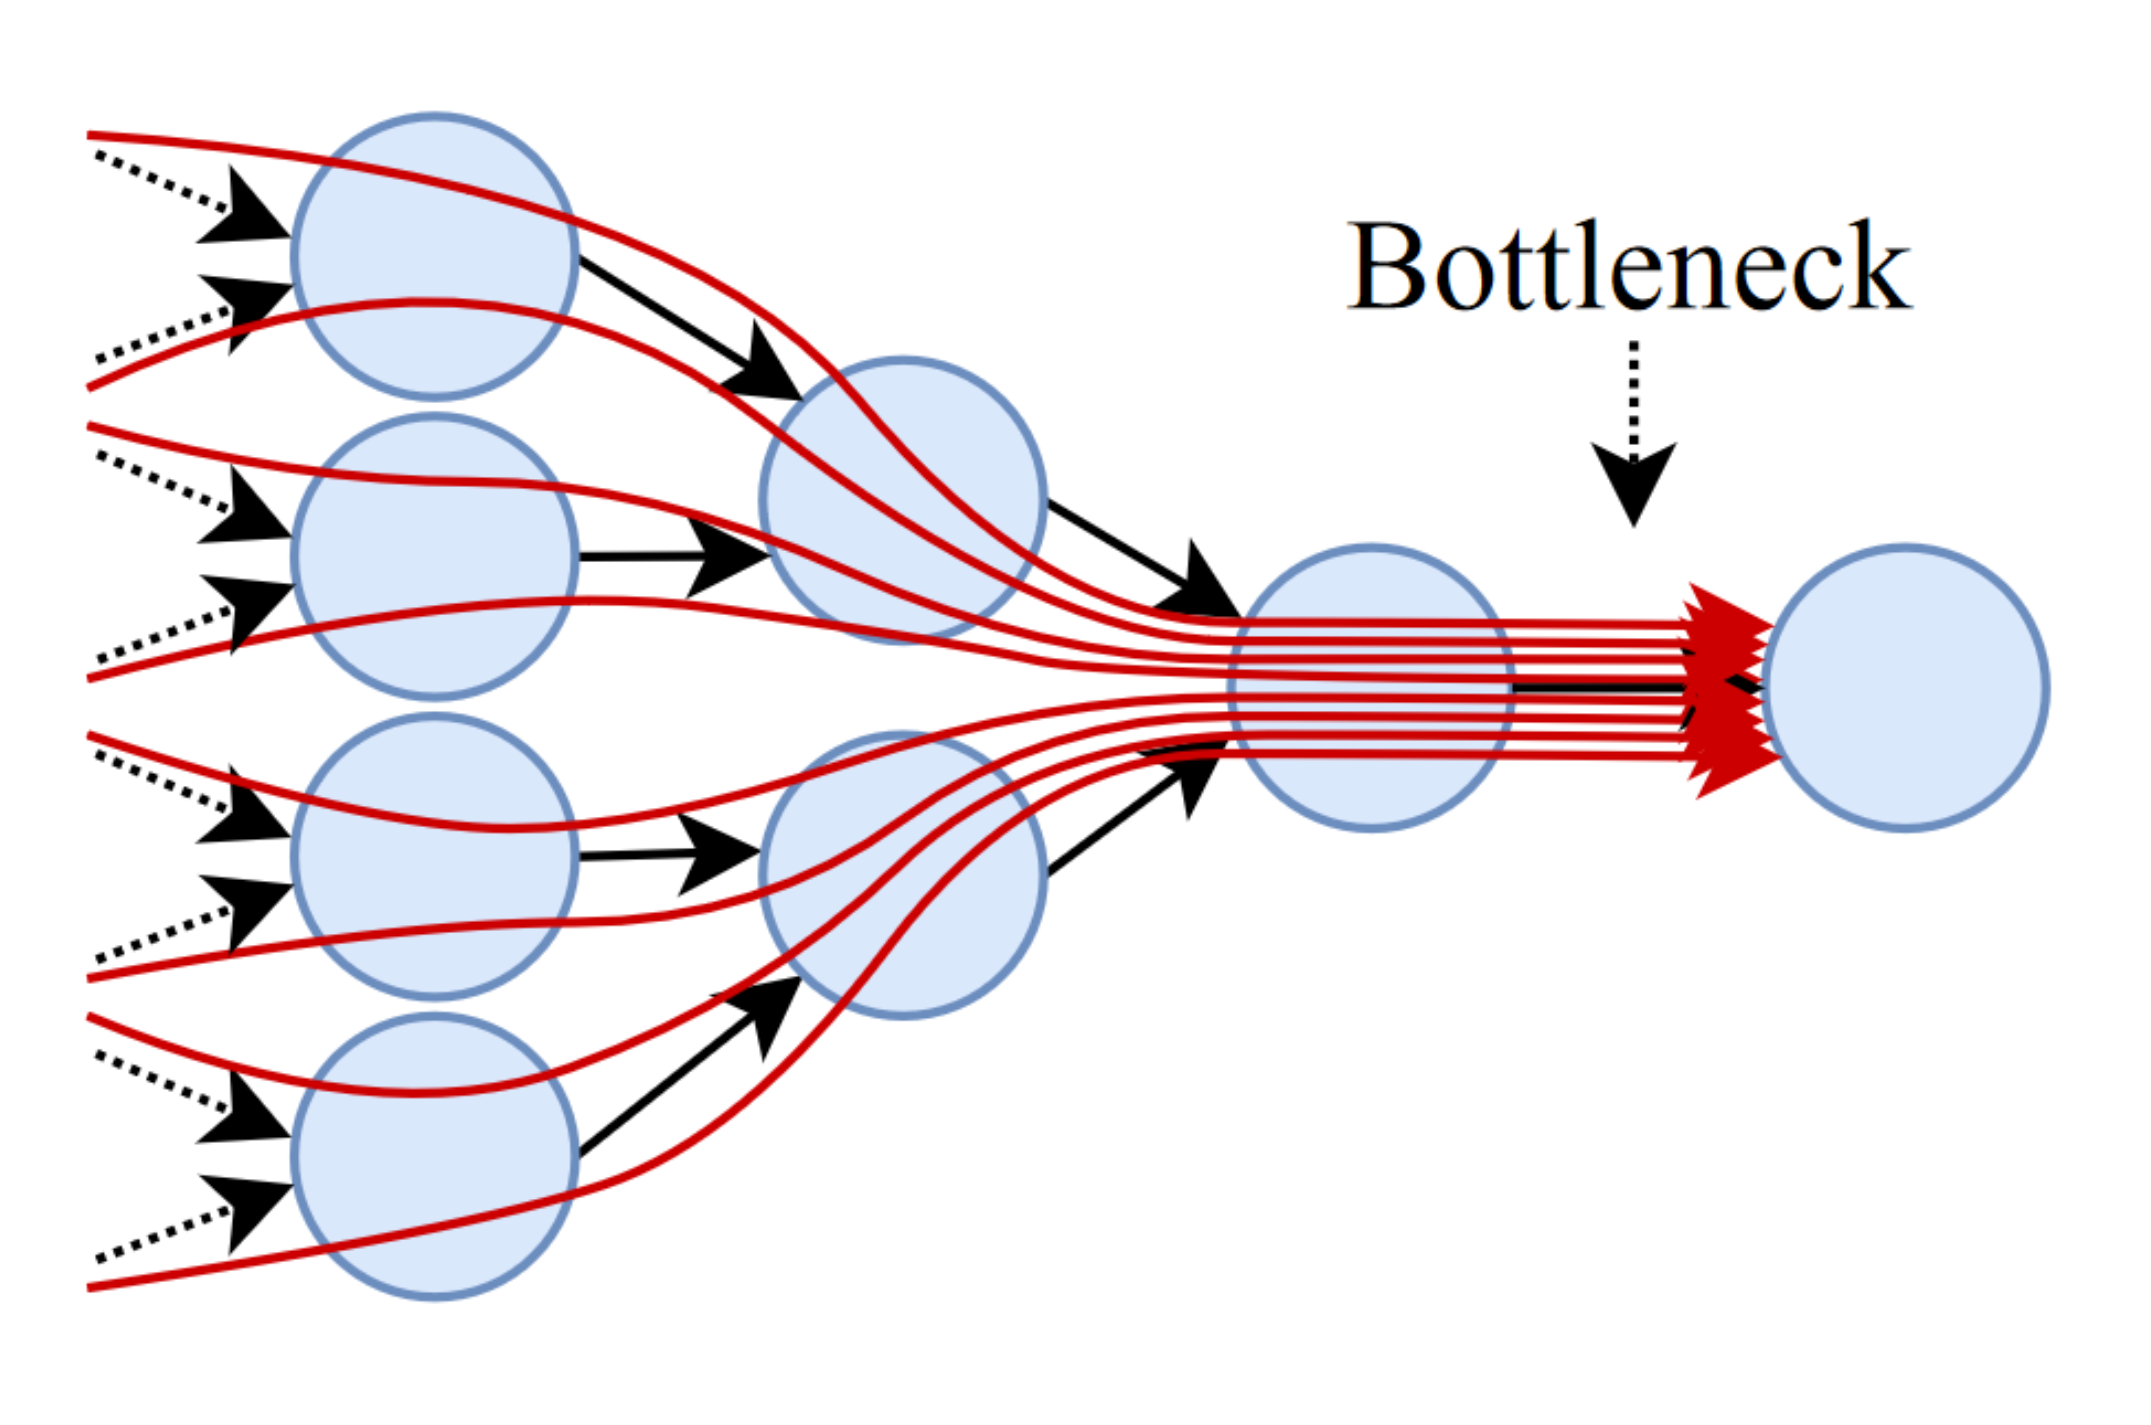
\includegraphics[width=0.75\textwidth]{img/bottleneck.png}
    \caption{Too much information is aggregated into a feature vector of a single node, resulting in information loss. \cite{alon2021bottleneck}}
    \label{fig:bottleneck}
\end{figure}

Both behaviours prevent GATs to improve by simply stacking hundreds of layers. However, there is an important distinction to make with regard to the degree to which this is problematic. In some uses cases, attending short-range neighborhoods already provides all necessary information and more distant information would not contribute to the outcome. A typical example are social networks, where link predictions only rely on connections that are a few hops away. Accordingly, GATs are well suited to solve short range taks and would not benefit from more distant information in the first place. However, there are problems which depend on long-range node interactions. Chemical properties of a molecule can depend on atoms on opposite sites of it, making it important to propagate this information by adding more layers \cite{alon2021bottleneck}.
\bigskip